%!TEX root = ./Body.tex

\chapter{Überblick Framework} % (fold)
\label{cha:Ueberblick_Framework}


\section{Arbeitsumgebung} % (fold) 
\label{sub:Arbeitsumgebung}
blablabla\\

blablabla
% section Arbeitsumgebung (end)


\section{Setup} % (fold) 
\label{sub:Setup}
blablabla\\

blablabla
% section Setup (end)


\section{CarMaker/Apo-Client Anpassungen} % (fold) 
\label{sub:Carmaker_Apo_Client_Anpassungen}
CarMaker ist eine von IPG Automotive \footnote{http://www.ipg.de} entwickelte Software, welche eine umfassende Simulation der Fahrzeugdynamik von Automobilen bietet. In unserem Versuchsaufbau ist diese Software für die Kommunikation mit dem Fahrsimulator und der Realisierung der Streckenführung zuständig.
Der ApoClient bietet uns eine ROS Schnittstelle zum CarMaker, sodass wir auf alle vom CarMaker empfangenen Daten auch über ROS zugreifen können.

Für unsere Problemstellung ist allerdings nicht nur ein Empfangen der Daten notwendig, sondern auch ein Übermitteln, da die drei Zielgrößen in Echtzeit übermittelt werden sollen. CarMaker und ApoClient wurden also so angepasst, dass sie in jedem Zeitschritt auch die Werte der drei Zielgrößen empfangen und an das Automobil weitergeben.

Die anfängliche Abtastrate des Systems betrug beim Projektstart nur 4-5 Hz. Bei dieser niedrigen ist eine vollständige Rekonstruktion der Lenkbewegung nur schwer möglich, weil der Fahrsimulator die übermittelten Werte direkt exakt einstellt und somit keine natürliche und flüssige Lenkbewegung ausführt. Durch eine höhere Abtastrate wird diese Lenkbewegung wieder vollständiger und somit für die weitere Verarbeitung nützlicher.
Um eine höhere Abtastrate zu erhalten wurden zwei Änderungen an dem System vorgenommen. Zum Ersten wurden alle relevanten Daten in einem ROS-Topic gebündelt, sodass nicht mehr 5 Topics veröffentlicht werden müssen. Dies bringt allerdings nur eine kleine zeitliche Verbesserung und wurde hauptsächlich wegen der Übersichtlichkeit vollzogen. Die zweite Änderung war eine Reduktion der abgefragten Daten auf die für uns relevanten Daten und somit eine erhöhte Abtastrate.

Insgesamt wurde die Abtastrate von 4-5 Hz auf konstante 15 Hz erhöht und eine bidirektionale Kommunikation in Echtzeit mit dem System ermöglicht.
% section Carmaker_Apo_Client_Anpassungen (end)


\section{Framework} % (fold) 
\label{sub:Framework}
Im Rahmen des Praktikums wurde ein Framework entwickelt, dessen Aufgabe darin bestand, Routineaufgaben zu automatisieren und eine einheitliche Plattform für die einzelnen Ansätze zum autonomen Fahren zu bieten. Die hier bereitgestellten Funktionalitäten waren die Voraussetzung für die Datensammlung und alle weiterführenden Experimente, daher wurden knapp zwei Drittel der zur Verfügung stehenden Zeit für die Entwicklung eingesetzt.

\begin{figure}[!h]
	\centering
	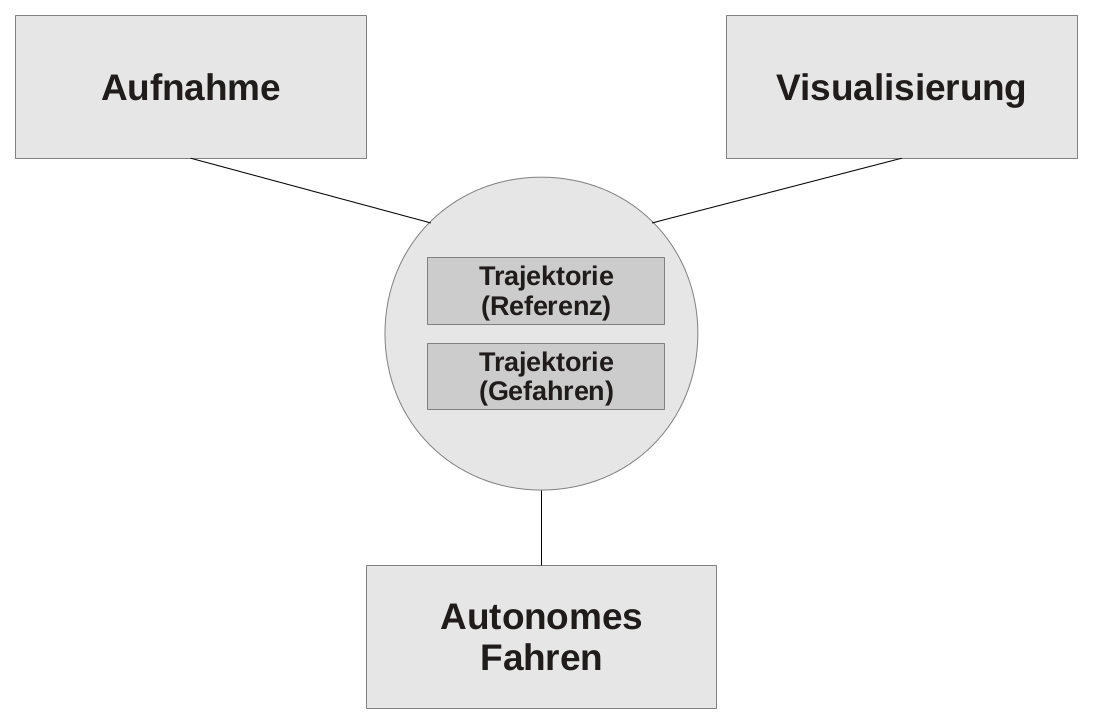
\includegraphics[scale=1.0]{images/framework/Framework Komponente.png} 
	\caption{Die einzelnen Komponenten den Frameworks.}
	\label{fig:FrameworkKomponente}
\end{figure}

Das Framework arbeitet auf Basis des \textit{Robot Operating System (ROS)} \footnote{www.ros.org} und besteht im wesentlichen aus zwei Programmen. Das als \textit{MLCore} bezeichnete Kernsystem umfasst die Aufnahme und Verwaltung von Fahrdaten, unterschiedliche Visualisierungen und das autonome Fahren (siehe Abbildung \ref{fig:FrameworkKomponente}). Das zweite Programm \textit{MLControl} dient zur Steuerung und greift hierzu auf die vom Kernsystem zur Verfügung gestellten Schnittstellen zu. Im folgenden Text werden die einzelnen Komponenten des Kernsystems näher erläutert.

\subsection{Ablaufsteuerung}
\label{subsec:Ablaufsteuerung}
Die Steuerung der internen Abläufe erfolgt über einen endlichen Automaten. Beim Entwurf wurde darauf geachtet, die Konfiguration des Kernsystems in den jeweiligen Zuständen zu konfigurieren. Dies erleichtert die Konfiguration und verringert die Fehleranfälligkeit.

\subsection{Aufnahme und Datenhaltung}
\label{subsec:AufnahmeUndDatenhaltung}
Wird eine Aufnahme gestartet, so nimmt das Kernsystem bis zu 15 mal pro Sekunde Nachrichten vom APO-Client entgegen. Jeder Datensatz enthält eine Reihe von Kennzahlen, die Informationen zum Fahrzeug liefern. Es werden ein Index sowie einige elementare Kennzahlen (wie z.B. die Ausrichtung des Fahrzeugs) ergänzt, anschließend erfolgt die Ablage in einer Liste im Hauptspeicher.

Die Liste kann über einen entsprechenden Befehl auf der Festplatte abgespeichert werden. Von da auch kann sie als Referenz erneut geladen werden oder für das Training der Lernverfahren verwendet werden.

\subsection{Visualisierung}
\label{subsec:Visualisierung}
Es werden zwei Modi zur Verfügung gestellt um die vorgegebene Referenz-Trajektorie und der vom Fahrzeug abgefahrenen Trajektorie grafisch darzustellen. Die Visualisierung erfolgt über RVIZ, ein zu ROS gehörendes, vielseitig einsetzbares Werkzeug.

\begin{figure}[!h]
	\centering
	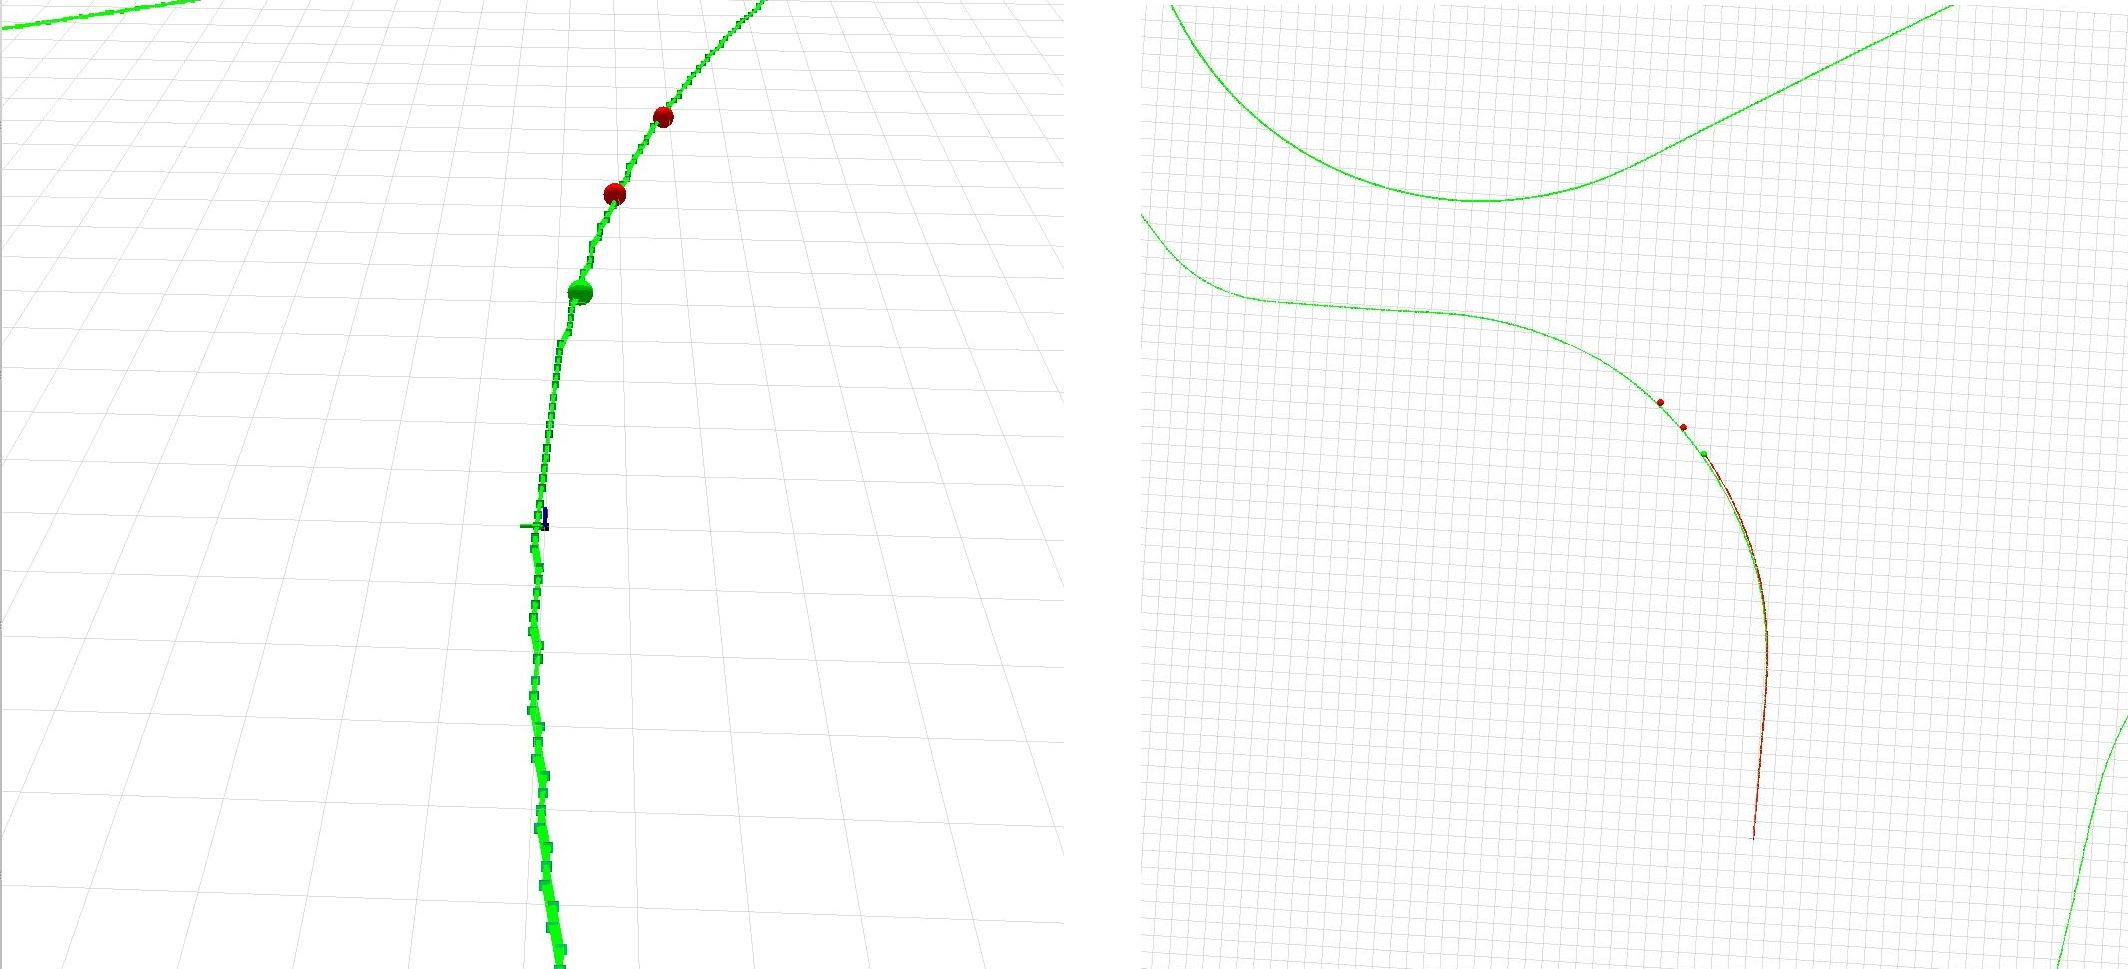
\includegraphics[scale=1.0]{images/framework/Visualisierungen.png} 
	\caption{Die beiden Visualisierungen "Gesamtüberblick" und "Fahrersicht" (von li. nach re.)}
	\label{fig:Visualisierungen}
\end{figure}

Der Modus Gesamtüberblick zeichnet sowohl Referenz als auch Fahrt bis zum aktuellen Zeitpunkt. Die Ansicht kann genutzt werden, um sich einen Überblick zu verschaffen und beide Trajektorien zu vergleichen.

Im Modus Fahrersicht wir die Referenz aus Sicht des Fahrzeugs visualisiert. Eine Reihe von Kugeln gibt an, an welchem Punkt sich der Fahrer gegenwärtig bzw. in naher Zukunft befinden muss. Diese Ansicht hat sich als die beste Möglichkeit zum Abfahren einer Trajektorie erwiesen. Abbildung \ref{fig:Visualisierungen} zeigt beide Modi.

\subsection{Autonomes Fahren}
\label{subsec:AutonomesFahren}
Die letzte Komponente beinhaltet die von den Praktikumsteilnehmern implementierten Lernverfahren. Über einen Auswahlmechanismus kann zur Laufzeit ein beliebiges Verfahren ausgewählt werden. Zu Testzwecken steht ein spezieller Ansatz zur Verfügung, der die Stellgrößen der Referenz weitergibt.
% section Framework (end)


\section{Toolbox} % (fold) 
\label{sub:Toolbox}
Das Toolbox-Paket enthält eine Reihe von Werkzeugen, die im Lauf des Praktikums entwickelt wurden. Sie ermöglichten es, weite Teile der anfallenden Arbeiten zu automatisieren. Hierdurch wurden Routineaufgaben, Experimente und die Analyse der Daten stark vereinfacht.
Alle Programme sind über die Konsole auszuführen und zeigen eine ausführliche Anleitung, wenn sie ohne Parameter aufgerufen werden. 

\subsection{Extraktion der Merkmale}
\label{subsec:ExtraktionDerMerkmale}
Die mit der Aufnahme-Funktion des Frameworks aufgezeichneten Fahrten sind als Rohdaten zu betrachten, die zuallererst veredelt werden müssen. Zwar können einige Kennzahlen bereits als Features verwendet werden, andere Features jedoch müssen erst auf Basis der Rohdaten berechnet werden.

Diese Aufgabe übernimmt das \textit{Extraktor}-Programm. Es wandelt die Rohdaten in eine Sequenz von Feature-Vektoren um; für jeden Datensatz in den Rohdaten wird ein entsprechender Feature-Vektor erzeugt. Außerdem wird eine Normalisierung durchgeführt, bei der alle Daten in ein Intervall von $[0,1]$ bzw. $[-1,1]$ überführt werden. Ausreißer werden ebenfalls behandelt.

Das Skript \textit{compileFeatureList.sh} nutzt den Extraktor, um alle vorliegenden Referenz-Fahrt-Paare zu konvertieren, zu konkatenieren und an zentraler Stelle abzulegen. Von hier aus kann eine weitere Verarbeitung stattfinden.

\subsection{Aufbau des Featureraums}
\label{subsec:AufbauDesFeatureraums}
Für die einzelnen Lernverfahren wurden unterschiedliche Programm-Bibliotheken eingesetzt. Da diese auch ihre eigenen Einlesefunktionen mit sich brachten, musste die im letzten Abschnitt beschriebenen Feature-Liste in unterschiedlichen Formaten verfügbar sein.

Das Programm Konverter wurde zur Umwandlung der Feature-Liste in andere Formate entwickelt. Eine wichtige Zusatzfunktion ist die gezielte Auswahl. Nur Features, die explizit angefordert werden, finden ihren Weg in die konvertierte Liste. So kann – quasi über die Kommandozeile – der Eingaberaum des Lernverfahrens strukturiert werden.

Es wurden von den Praktikumsteilnehmern unterstützende Bash-Skripte geschrieben, die im Rahmen des Trainings der Lernverfahren auf den \textit{Konverter} zurückgreifen.

\subsection{Aufteilung in Untermengen}
\label{subsec:AufteilungInUntermengen}
Beim maschinellen Lernen ist es üblich, die gesammelten Daten in mehrere Teilmengen aufzuteilen, die dann unterschiedlichen Zwecken (wie z.B. dem Training oder der Evaluation) dienen. Das \textit{Remixer}-Programm führt genau diesen Arbeitsschritt durch.

Es arbeitet auf Zeilenebene; es liest eine Datei zeilenweise ein, teilt die Zeilen zufällig auf die einzelnen Sets auf und legt diese dann als Datei auf der Festplatte ab. Dieser Ansatz erlaubt es, auf Basis von bereits konvertierten Datensätzen (siehe vorheriger Abschnitt) zu arbeiten.

Größe und Anzahl der Sets sind fest im Programm kodiert, es können jedoch per Kommandozeile unterschiedliche Konfigurationen ausgewählt werden. Das Programm findet unter anderem im Rahmen der Evaluation Anwendung.

\subsection{Visualisierung}
\label{subsec:Visualisierung}
Zum Auffinden von Korrelationen zwischen einzelnen Features wurden eine Reihe von Bash-Skripten geschrieben. Diese nutzen den Konverter, um die jeweils zu untersuchenden Features auszuwählen und in ein Format zu konvertieren, welches mittelt GnuPlot \footnote{www.gnuplot.info} visualisiert werden kann.
% section Toolbox (end)


\section{Visualisierung} % (fold)
\label{sec:Visualisierung}
blablabla

\subsection{Visualisierung1} % (fold)
\label{sub:Visualisierung1}
blablabla

% subsection Visualisierung1 (end)

\subsection{Visualisierung2} % (fold)
\label{sub:Visualisierung2}
Eigentlich kann man hier nichts schreiben außer das Bild machen und auf den Datenaufnahme abschnitt verweisen. Dort wird ja das Verfahren genauer erklärt.. ist sonst redundant.
% subsection Visualisierung2 (end)

% section Visualisierung (end)

% chapter Ueberblick_Framework (end)
